% ============================================================
\section{Screening for a Capability Worth Preserving}
\label{sec:forecasting}
% ============================================================

To ask whether fine-tuning damages valuable pre-trained features we first have
to find a cell where such features are demonstrably present.  This section
reports that search, and it comes out negative: across \textbf{32 screened
cells}---21 Moirai (three capacities, five datasets, two horizons), 5
Chronos-T5, 5 TimesFM-2.5 and 1 Moirai/ILI---\textbf{five} clear the value gate,
and all five are ETTh2 on Moirai.  Thirty-one of the 32 also carry a paired
frozen-encoder intervention; TimesFM/Electricity is screened but has no B/D
pair, so the intervention matrix has 31 rows throughout.
Figure~\ref{fig:screen} shows both: the screen emptying, and the gate running
backwards on the cells that clear it.

\begin{figure}[t]
\centering
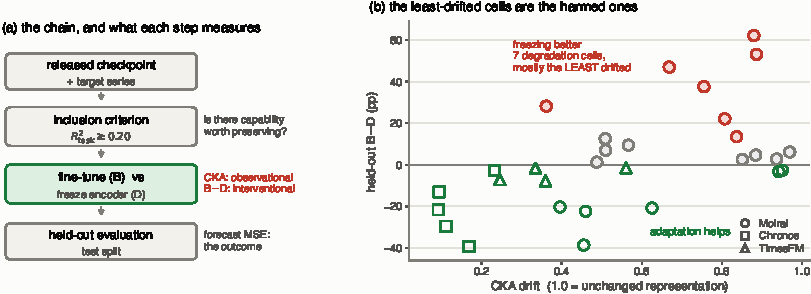
\includegraphics[width=\linewidth]{fig1_diagnostic_flow.pdf}
\caption{\textbf{(a) The screen empties.} Of 32 screened cells, five clear
$R^2_\text{task}(\text{PT}){\geq}0.20$ and \emph{none} satisfies the
three-clause degradation definition of \S\ref{sec:method}; three of the five
survivors are \emph{improved} by full fine-tuning.  \textbf{(b) The gate points
the wrong way.}  The 31 cells with a paired frozen-encoder run, plotted as gate
score against held-out $\text{B}{-}\text{D}$ (positive ${=}$ freezing better,
so the upper-right quadrant beyond the dashed threshold is the only region a
degradation cell could occupy).  Within Moirai---the only backbone with enough
cells to ask, and pooling across backbones is what \S\ref{sec:forecasting:nonmoirai}
forbids---higher measured pre-trained value predicts encoder adaptation helping
\emph{more} ($\rho{=}{-}0.52$), while CKA drift does not reliably order them
($\rho{=}{+}0.17$, series CI $[-0.47,{+}0.72]$).  Both correlations are
directions rather than interval claims (Appendix~\ref{app:clustered}).
Filled markers clear the gate.
Every value is read from \texttt{scripts/cell\_matrix.py}; the figure asserts
each count quoted here at draw time and fails loudly if the run records move,
so it cannot silently disagree with the text.}
\label{fig:screen}
\end{figure}

% ============================================================
\subsection{The Screen}
\label{sec:forecasting:gate}
% ============================================================

Setup follows \S\ref{sec:method}: $h{\in}\{96,192\}$ for Moirai and $h{=}24$
elsewhere, $n{=}500$ or $n{=}1{,}000$ samples, 3--10 seeds per cell.  Every gate
value is computed on held-out test windows against a lookback-96 ridge map fit
on the cell's own training split.

\textbf{Moirai: 5 of 21} (Appendix Table~\ref{tab:r2task}).  The five are
ETTh2 at Small $h{=}96$ ($+0.400$) and $h{=}192$ ($+0.464$), Base $h{=}96$
($+0.361$) and $h{=}192$ ($+0.275$), and Large $h{=}96$ ($+0.219$).  Every
other dataset fails at every capacity: ETTh1 spans $-0.243$ to $-0.501$,
Weather $-0.621$ to $-1.324$, \texttt{Electricity7} $-0.085$ and $-0.047$, and
ETTm2 $-0.110$ to $+0.108$---never reaching the threshold even where the sign
turns.  Capacity does not help: Moirai-Base is 6.3$\times$ larger than
Moirai-Small and \emph{further} behind the baseline on both ETTh1 and Weather.

\textbf{Chronos-T5-Small: 0 of 5} and \textbf{TimesFM-2.5: 0 of 5}
(\S\ref{sec:forecasting:nonmoirai}, Appendix Table~\ref{tab:crossbackbone}).
Across the ten cells the scores run from $-1.281$ (ETTm2) to $+0.132$
(Electricity), per cell in Appendix Table~\ref{tab:crossbackbone}.
The two backbones agree on the ordering of the five datasets
despite unrelated pre-training corpora and architectures, which is what one
expects if the ranking is a property of the \emph{benchmarks} rather than of
either model.  Note in particular that ETTh2---the only dataset on which
Moirai clears the gate---is where Chronos posts its second-worst score.
The advantage is not a property of the dataset alone.

\textbf{ILI: $-1.625$.}  Moirai-Small's zero-shot MSE on ILI is $2.6\times$ the
fitted baseline's; an earlier public version reported this cell as a $57\%$
gate-\emph{pass}, and that number is withdrawn (Appendix~\ref{app:ili_gate}).

\textbf{Why the estimator matters more than the threshold.}
Moving the threshold anywhere in $[0.10,0.60]$ changes which cells pass but
changes nothing below (\S\ref{sec:analysis:prospective}).  Changing the
\emph{baseline} changes everything.  Swapping the fitted regression for the
per-window trend extrapolation an earlier version used---a denominator a
constant predictor beats---moves 17 cells across the threshold
(Appendix~\ref{app:gatecorrection}).  Across five estimators on the same
windows and the same numerator, the count clearing $0.20$ with a denominator no
worse than predicting the training mean is 5, 4, 2, 4 and 7 of 32: the screen's
emptiness is not one estimator's artefact.  The passing \emph{sets}, however,
are nearly disjoint---all five ETTh2 survivors fail against a seasonal-naive
baseline and against a univariate AR map---so five cells clear \emph{this} gate
(Appendix~\ref{app:baselines}).

% ============================================================
\subsection{What Fine-Tuning Does to the Five Survivors}
\label{sec:forecasting:results}
% ============================================================

The five gate-passing cells are the entire evidence base for a claim about
damage to valuable features, and they do not support one
(Appendix Table~\ref{tab:gate_survivors}).

\textbf{On three of the five, full fine-tuning is a large improvement.} On
Moirai-Base at $h{=}96$ and $h{=}192$ and Moirai-Large at $h{=}96$,
forgetting is $-31.4\%$, $-36.3\%$ and $-42.4\%$ against zero-shot, negative
in 3/3 seeds each, at CKA $0.460$, $0.396$ and $0.626$.  These are the
cells with a demonstrated pre-trained advantage \emph{and} the largest
representational change among the five, and fine-tuning them cuts MSE by
roughly a third.  Freezing the encoder captures only part of that gain
($-9.1\%$, $-16.1\%$, $-21.6\%$), so encoder adaptation is where most of the
improvement comes from.

\textbf{On the remaining two, the mean harm does not survive inspection.}
Moirai-Small/ETTh2 at $h{=}192$ reads forg.$_\text{B}{=}{+}1.99{\pm}3.32$
with 5 of 10 seeds positive---a coin flip on the sign, and the one cell in the
matrix that comes closest to degradation.  At $h{=}96$ the cell mean is
$+9.71{\pm}10.58$ with 4 of 10 seeds positive, and that mean is produced by a
single seed: seed 42 diverges to $+98.9\%$ under full fine-tuning and to
$+91.1\%$ under the \emph{frozen} encoder, so it is a training failure and not
an encoder-drift effect.  Dropping it leaves
forg.$_\text{B}{=}{-}0.20{\pm}4.15$ over 9 seeds (3 positive) and
forg.$_\text{D}{=}{-}2.45{\pm}0.16$.  We report the cell means including seed
42 everywhere in this paper, and note the decomposition here so the reader can
see what the mean is made of.

\textbf{Consequence.}  There is no cell in this matrix where we can say that
fine-tuning reliably destroyed a demonstrated pre-trained capability.
\S\ref{sec:analysis:degradation} states that verdict against the three-clause
definition and reports what it costs the diagnostic we proposed.

% ============================================================
\subsection{Sample Size, and What Mitigation Is For}
\label{sec:forecasting:replication}
% ============================================================

Sweeping $n{\in}\{500,\ldots,10\mathrm{k}\}$ on Moirai-Small/ETTh2 at $h{=}96$
---one of the five survivors, so a sweep where a pre-trained advantage does
exist---separates the two readings directly: drift grows monotonically with $n$
(CKA $0.949$ at 500 to $0.518$ at 10k) while forgetting is non-monotonic and
reverses sign, $+14\%$ at 500, $-2.9\%$ by 2k, $-5.3{\pm}6.2\%$ at 10k (7/10
negative). \textbf{If drift magnitude predicted harm these columns would track;
they do not.}  Whatever harm exists is confined to Small at $n{\leq}1$k, which
is also where the sweep's seed variance is largest
(Table~\ref{tab:sample_sweep}, Figure~\ref{fig:dissociation} and
Appendix~\ref{app:n5k_trajectories} for the bimodal $n{=}5$k cell and the
protocol comparison).  This sweep predates held-out scoring and is scored on one
split throughout, which is why its $n{=}500$ value ($+14.0{\pm}6.7$) differs
from the held-out mean above ($+9.71{\pm}10.58$);
\S\ref{sec:analysis:heldout} is about exactly that gap.

\textbf{What mitigation is for.} Five strategies spanning unconstrained
fine-tuning to full freezing---LoRA, EWC, L2-SP, frozen encoder, strict
freeze---are reported in Appendix~\ref{app:full_tables}, on
Moirai-Small/ETTh2, the one cell where we ran the whole spectrum: weight
anchoring does not help there, LoRA does, and no six-condition comparison
exists for the other survivors.  But the screen bounds what any of it can be
for: on 27 of the 32 cells we screened there is no demonstrated advantage to
protect, and on three of the remaining five, unconstrained fine-tuning beats
zero-shot by 31--42\% and the frozen encoder by 20--22 points.

\textbf{Retracted: linear-probe analyses of this cell.} A $\Delta R^2$ probe
account of \emph{what} restructured stood here and is retracted
(Appendix~\ref{sec:retraction}; the withdrawn numbers and the re-run that
refutes them are kept in Appendices~\ref{app:probing},~\ref{app:layerunfreeze}
and~\ref{app:orthogonal}).  The
layer-wise \emph{task} readings survive, being forecast MSE: unfreezing the top
3 of 6 layers and unfreezing all 6 are indistinguishable on the task
($-5.9{\pm}2.0$\% against $-7.9{\pm}2.1$\%, SEM over 10 seeds each) while their
CKA differs by 3.5 standard errors ($0.716$ against $0.465$), so matching the
task outcome does not require matching the drift.
